%\documentclass{report}
%\usepackage[T1]{fontenc}
%\usepackage[utf8]{inputenc}
%\usepackage[francais]{babel}
%\usepackage{amsmath}
%\usepackage{graphicx}
%\usepackage[backend=biber,style=authoryear,bibencoding=utf8]{biblatex}
%\usepackage[colorlinks,linkcolor=blue]{hyperref}
%\newcommand{\micro}{$\mathrm{\mu}$}
%\addbibresource{biblio2.bib}
%
%
%\begin{document}
\chapter{De la cellule au muscle}


\begin{center}
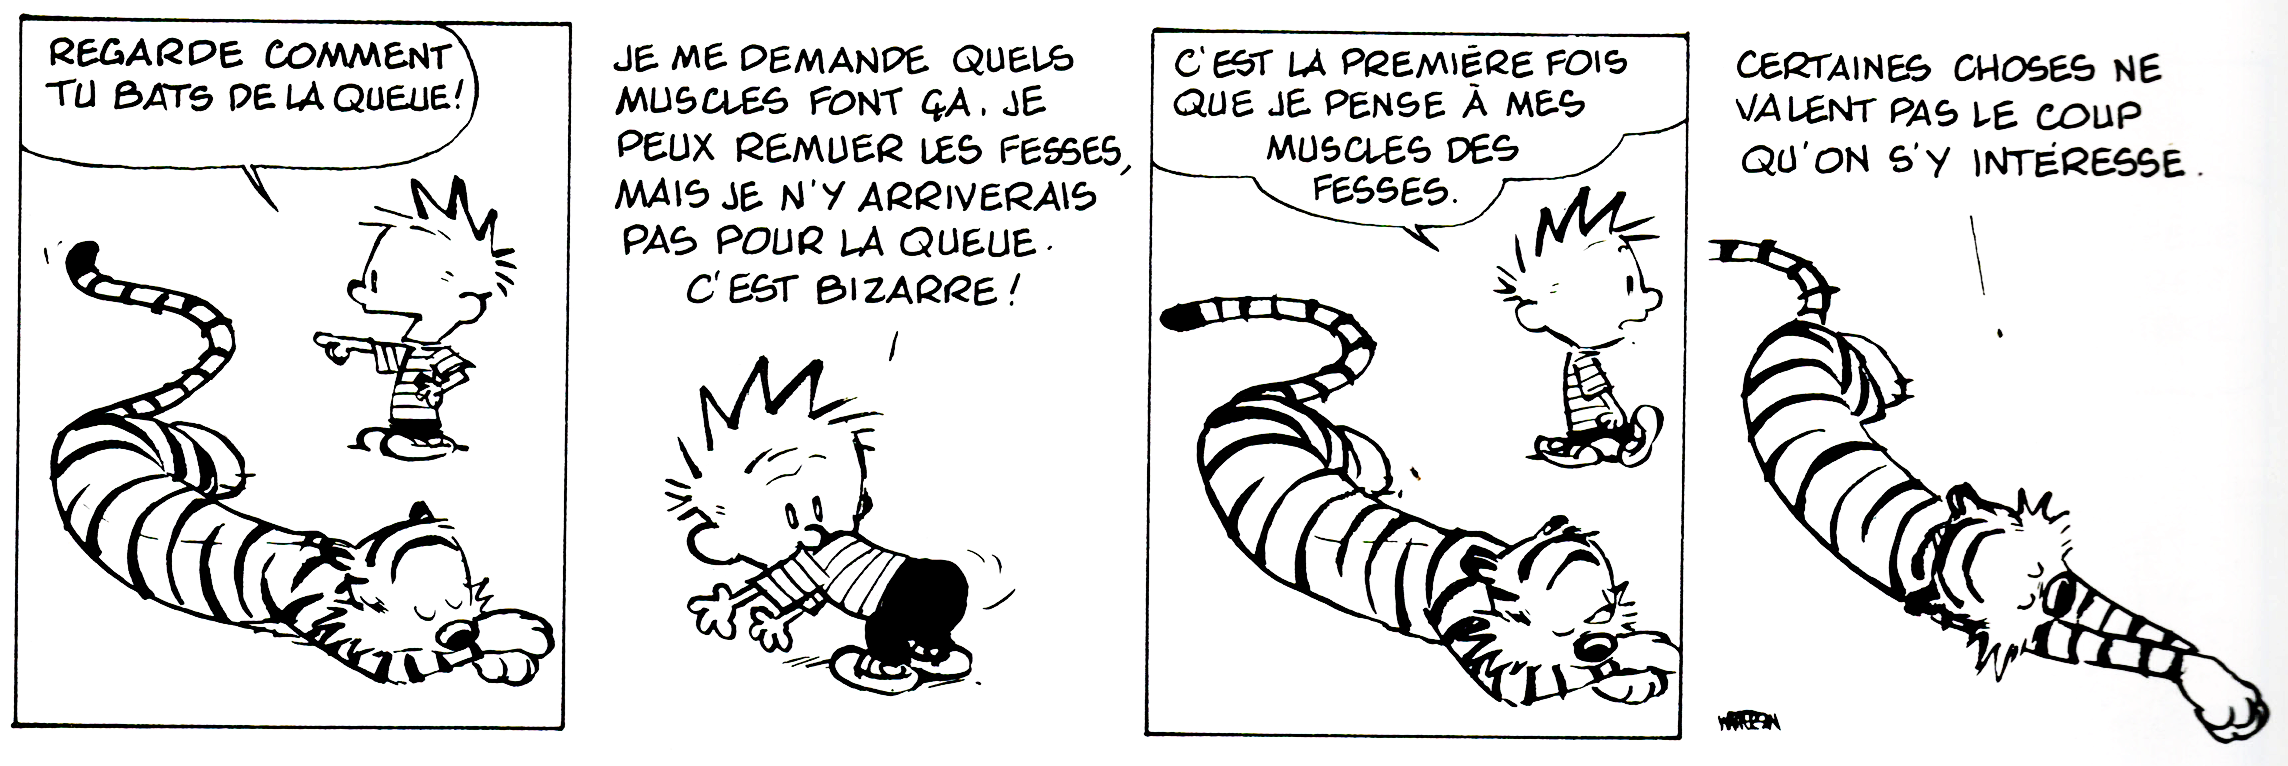
\includegraphics[scale=0.7]{Chapitre4.png}
\end{center}
\newpage

Les muscles représentent environ 40\% de la masse totale d'un humain adulte. Ils participent à tous les phénomènes indispensables à notre vie : ils nous permettent de nous mouvoir, d'exercer des forces sur notre environnement, mais aussi de respirer, de faire circuler le sang, de digérer \dots 
Il existe trois principaux types de muscles : lisses, cardiaque, et squelettiques. Les muscle lisses, comme ceux que l'on trouve le long du tube digestif ou des vaisseaux sanguins, mais aussi dans la vessie ou l'utérus, ne peuvent pas être contrôlés volontairement. 
Le muscle cardiaque, présent uniquement au niveau du c\oe ur, a une organisation spécifique qui lui permet de maintenir des contractions régulières et permanentes, assez puissantes pour faire circuler le sang dans le système circulatoire. 
Les muscles squelettiques sont les seuls que nous contrôlons volontairement. Comme leur nom l'indique, ils s'ancrent au squelette par l'intermédiaire des tendons, et ce sont eux qui nous permettent de bouger nos membres.  
Il en existe environ 640, de toutes tailles, des minuscules muscles contrôlant les mouvements des yeux à l'énorme quadriceps.

\section{Organisation du muscle squelettique}

Dans le chapitre premier, une cellule typique et peu différenciée a été présentée, semblable aux précurseurs du muscle. Les cellules qui composent les muscles ont une organisation bien différente. 
En partant des cellules et des protéines qui ont été décrites dans les chapitres précédents, nous allons décrire l'architecture du muscle. 

\subsection{Du myoblaste au myotube}

\begin{figure}
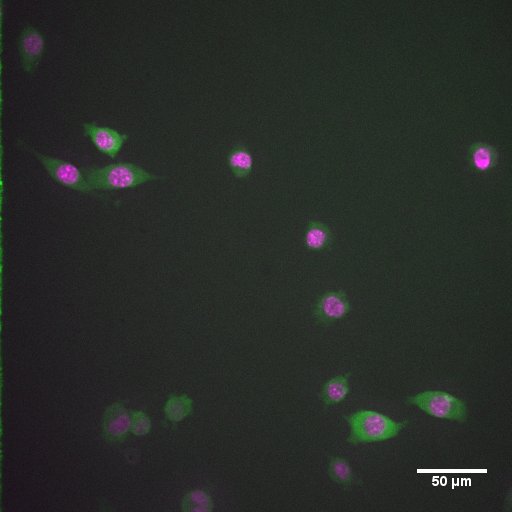
\includegraphics[scale=0.25]{Figures/Myocytes.png} 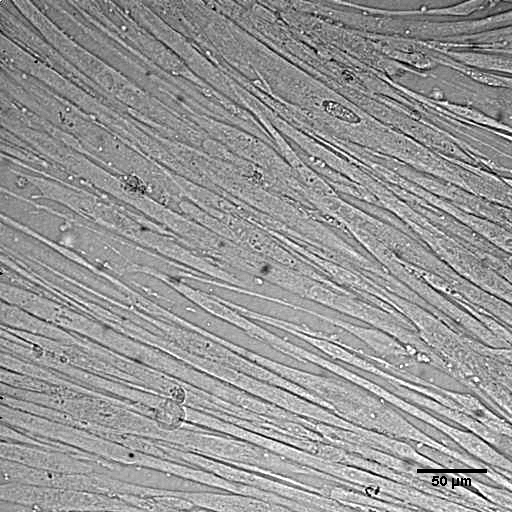
\includegraphics[scale=0.25]{Figures/Myotubes_flox_D4.png} 
\caption{Myoblastes primaires infectés avec un plasmide MRTF-A GFP, et myotubes obtenus à partir de myoblastes primaires après 4 jours de différenciation \textit{in vitro} par Alessandra Pincini. En magenta, le noyau marqué au DAPI, en vert MRTF-A GFP.}
\end{figure}


Les myoblastes sont les cellules progénitrices du muscle. Les C2C12 sont une lignée immortalisée de myoblastes murins, mais des myoblastes primaires peuvent également être mis en cultures \textit{in vitro}.
La différenciation se produit quand les myoblastes sont suffisamment nombreux et que les facteurs de croissance qui les maintiennent en prolifération viennent à manquer. 
%Les myoblastes se mettent alors à sécréter de la fibronectine, la liaison intégrine/fibronectine étant indispensable à la différenciation. 
%% Impossible de retrouver la référence
\begin{figure}
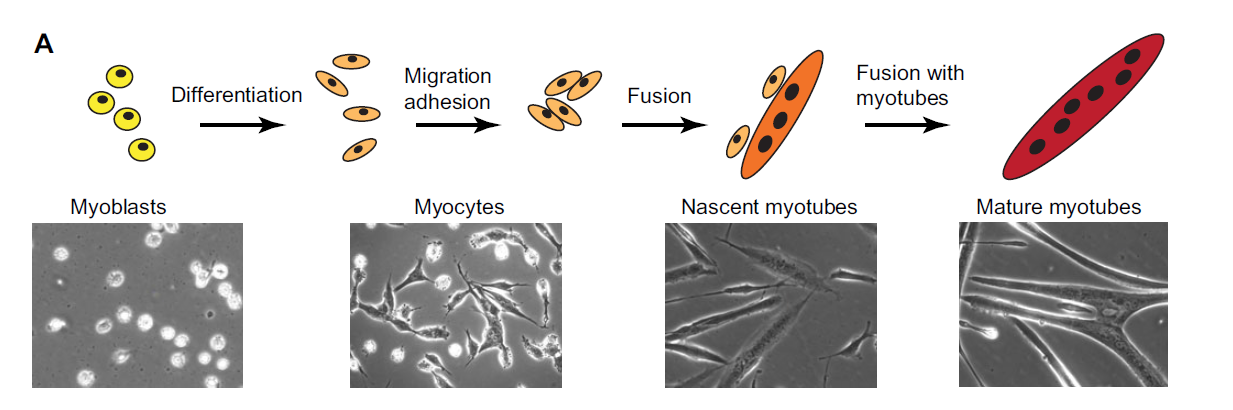
\includegraphics[scale=0.4]{Figures/Myoblast_fusion.png} 
\caption{\'Etapes successives de la différenciation des myoblastes en myotubes chez la souris, d'après \cite{abmayr_myoblast_2012}. }
\end{figure}

Les myoblastes vont alors s'aligner les uns avec les autres, sortir du cycle cellulaire et devenir des myocytes. Certains de ces myocytes deviendront des cellules fondatrices de myotubes. Les autres myocytes vont alors fusionner avec eux lors d'un processus asymétrique qui mène à la formation de myotubes polynuclés de plusieurs centaines de microns de long. 
Les myoblastes étendent autour d'eux des lamellipodes et des filopodes pour contacter les cellules voisines. Au niveau de ces contacts, les compositions en lipides de la membrane change, on trouve un grand nombre de protéines comme les M- et N-cadhérines, les intégrines et les filamines qui assurent un lien avec le cytosquelette (revue par \cite{abmayr_myoblast_2012}). Ce dernier est réorganisé localement : un réseau dense se forme sous la membrane, mis sous tension par la myosine 2A (\cite{duan_dependence_2009}). 
Le myoblaste envahit le myotube à l'aide de structures podosome-like quasiment exclusivement composées d'actine en filaments, avant que des pores se forment entre les deux cellules pour achever la fusion. 


\begin{figure}
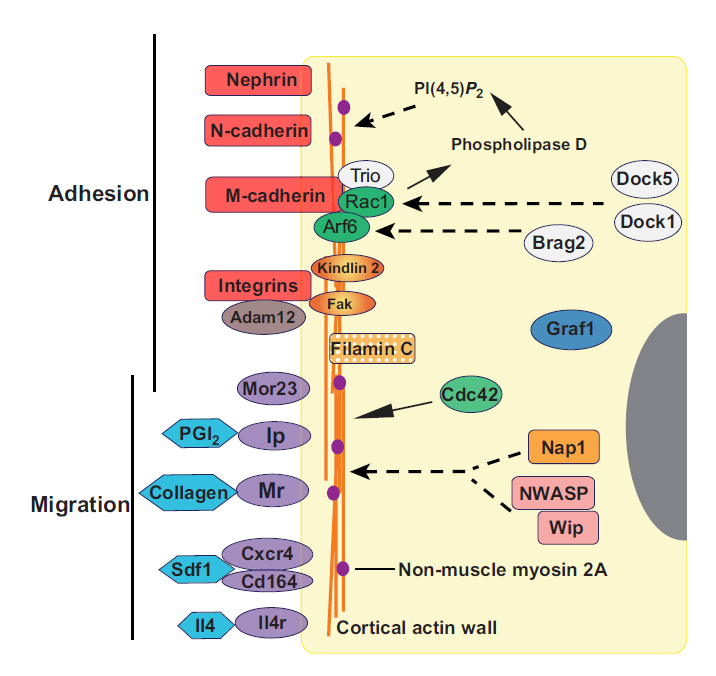
\includegraphics[scale=0.3]{Figures/Myoblast_pathways.png} 
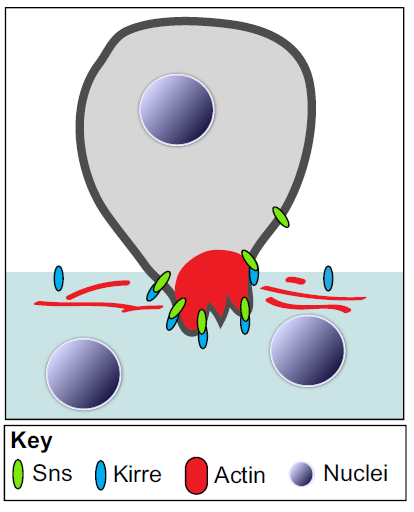
\includegraphics[scale=0.3]{Figures/Myoblast_invasion.png} 
\caption{Protéines impliquées dans la différenciation des myoblastes et invasion d'un myotube par un myocyte avant la fusion.}
\end{figure}

Une fois le myotube formé, il mature pour devenir une myofibre en développant une organisation spécifique de l'actine et de la myosine.




\subsection{Une organisation spécifique de l'actine et de la myosine }

À l'intérieur d'une myofibre totalement différenciée, l'actine est organisée en unités appelées les sarcomères. 

\begin{figure}[p]
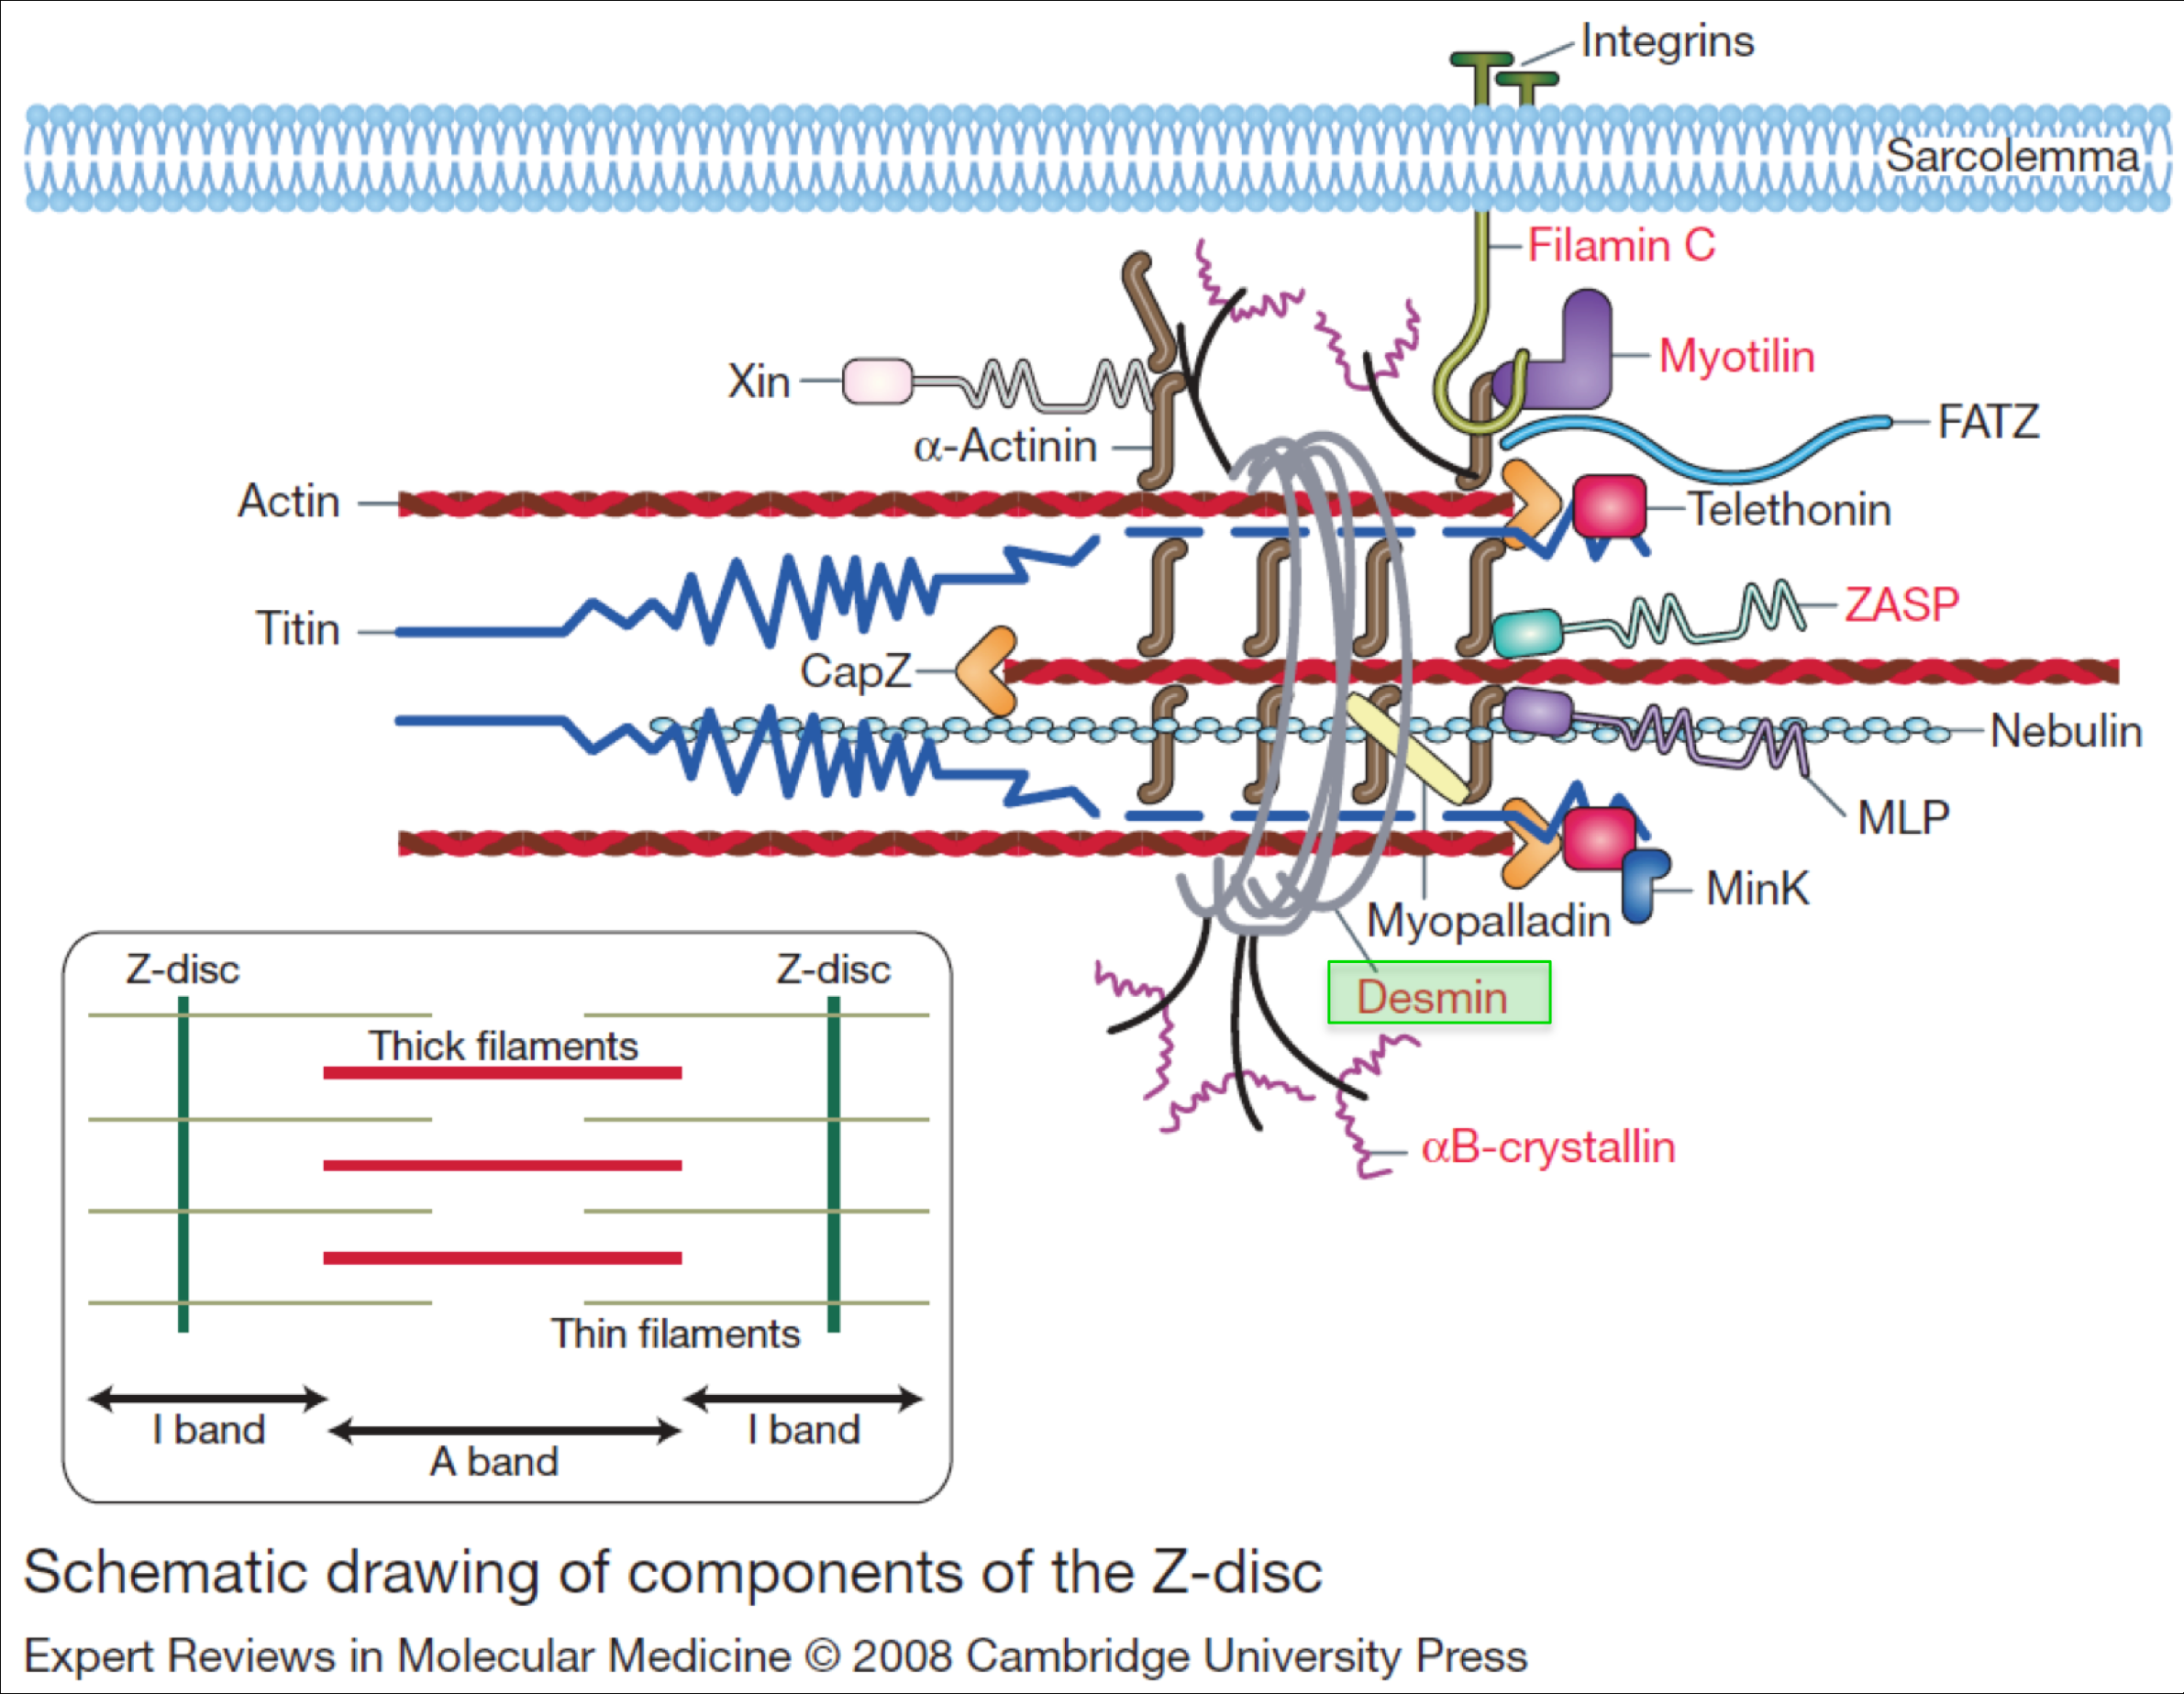
\includegraphics[scale=0.2]{Figures/sarcomere.png} 
\caption{Organisation schématique du disque Z, d'après \cite{ferrer_molecular_2008}}
\end{figure}

Un sarcomère est composé de filaments d'actine et de filaments de myosines qui sont dotés de milliers de têtes de myosines. Le mouvement des têtes de myosines sur le filament d'actine fait coulisser les deux filaments l'un par rapport à l'autre, ce qui crée la contraction musculaire. 

Afin que les filaments d'actine, dont nous avons vu au chapitre 2 qu'ils sont ordinairement très dynamiques, maintiennent leur taille, ils sont coiffés aux deux extrémités par CapZ d'un côté et par la tropomoduline de l'autre.
On pense que les nébulines, de très longues protéines qui peuvent se lier à environ 200 actines en filament, servent d'étalon pour fixer la longueur des filaments d'actine dans les sarcomères. 



\begin{figure}[p]
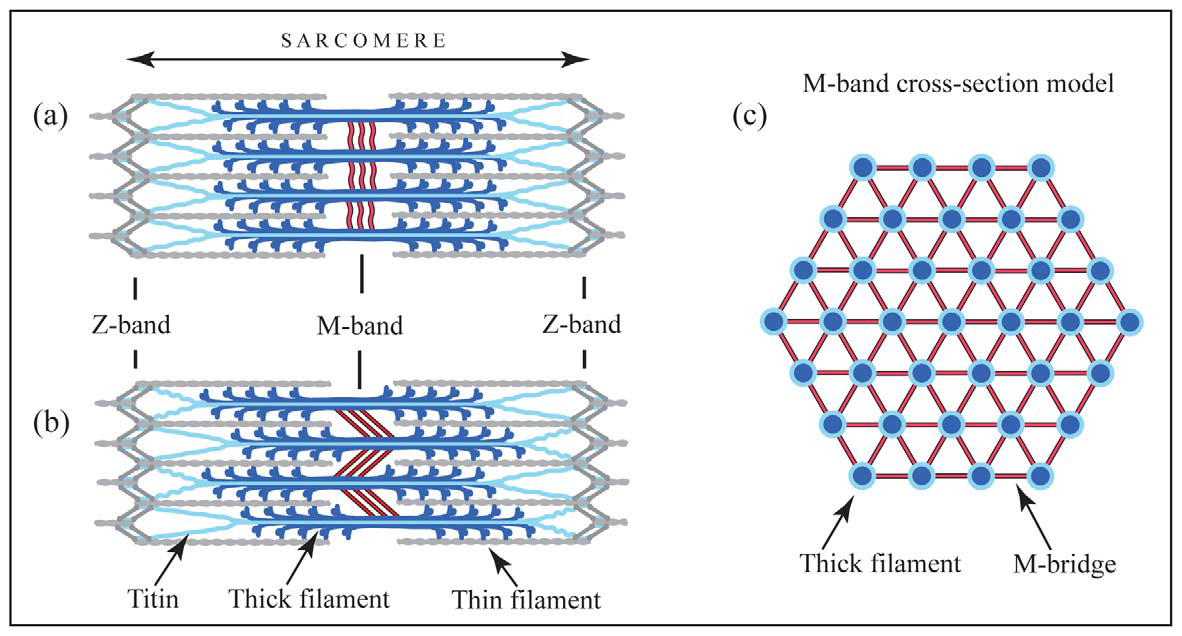
\includegraphics[scale=0.4]{Figures/Myomesine.png}
\caption{Organisation dans les deux plans des filaments de myosine au niveau de la bande M, d'après \cite{tskhovrebova_making_2012}}
\end{figure}
 
Autour des filaments d'actine, la tropomyosine, liée également à la troponine, régule la liaison entre le filament d'actine et le filament de myosine, en recouvrant ou découvrant les sites de liaison des têtes de myosines à l'actine, et le maintient polymérisé. 

Les filaments de myosine sont maintenus alignés grâce à la structure de la bande M, et les filaments d'actine par le disque Z. 

Au niveau de la bande M, les filaments de myosine se lient aux protéines M, aux myomésines et aux titines. 
La titine est une protéine géante qui maintient l'intégrité du sarcomère en se liant à la bande M, au disque Z et aux filaments de myosine. Elle présente une structure enroulée sur elle-même, et fonctionne comme un ressort qui stocke de l'énergie quand le sarcomère change de longueur, et contribue ainsi à maintenir l'intégrité de l'ensemble de la structure. 
Les myomésines ont une structure semblable mais sont plus courtes. Elles forment des ponts entre les filaments de myosines pour les maintenir dans une structure qui ressemble à un réseau hexagonal. 

Au niveau du disque Z, un grand nombre de protéines viennent assurer l'ancrage des filaments d'actine et l'organisation du sarcomère. Une partie d'entre elles est également partie prenante de cascades de signalisation.
L'$\alpha$-actinine, déjà évoquée précédemment en tant que protéine liée à l'actine, assure vis-à-vis de l'actine la même mission que les myomésines pour les filaments de myosine : elle lie les filaments entre eux pour former un réseau hexagonal, et lie également les titines. 
Par l'intermédiaire de la filamine C, l'$\alpha$-actinine relie les filaments d'actine du sarcomère aux intégrines qui assurent l'ancrage avec la matrice extra-cellulaire. 
La desmine, le filament intermédiaire du cytosquelette spécifique du muscle s'enroule autour du disque Z pour maintenir sa structure, et l'$\alpha$B-cristalline l'empêche de former des agrégats. 


\subsection{Rôle de la voie RhoA/MRTF-A/SRF}

Parmi les gènes cibles de SRF, on trouve un grand nombre de protéines indispensables à la constitution des sarcomères :  tous les différents gènes d'actine et en particulier l'$\alpha$ Skeletal Actin , des myosines (MHC9,myo16,myoIE), des $\alpha$-actinines, des intégrines et des tropomyosines (\cite{selvaraj_megakaryoblastic_2003},\cite{charvet_new_2006},\cite{esnault_rho-actin_2014}).

MyoD, facteur de transcription de la famille des Myogenic Regulatory Factors et marqueur de la différenciation en cellule musculaire, contient un Serum Response Element (\cite{lhonore_myod_2003}) et est activé par MRTF-A/SRF (\cite{mokalled_mastr_2012}). 

Il suffit qu'un seul des maillons de la voie RhoA/MRTF/SRF manque pour que la différenciation en cellule musculaire échoue. 

\textit{In vivo} dans des souris ayant une délétion conditionnelle de SRF dans les muscles, on observe une diminution de l'expression de la tropomyosine et de l'$\alpha$ actine du muscle squelettique, corrélés à des défauts dans la croissance des myofibres, une désorganisation des sarcomères et une hypotrophie musculaire (\cite{charvet_new_2006},\cite{li_requirement_2005}). 

Les souris dominant négatif MRTF-A sont viables mais présentent une hypotrophie musculaire qui dépend du niveau d'expression de MRTF-A, une fibrose, et des noyaux positionnés au centre des fibres musculaires, ce qui les désorganise \parencite{li_requirement_2005}. \textit{In vitro}, la différenciation des C2C12 nécessite également la présence des MRTF \parencite{selvaraj_megakaryoblastic_2003}, de SRF et de RhoA (\cite{wei_rhoa_1998}). 

\cite{kawauchi_p130cas-dependent_2012} détaillent un peu plus ces voies de signalisation impliquées dans la différenciation musculaire, en montrant que la signalisation passe par p130Cas, les intégrines $\beta$3 et ILK, qui désactivent à la fois ERK1/2 (ce qui empêche la phosphorylation de MRTF-A et donc promeut son accumulation nucléaire, et met hors-jeu les TCF), et la cofiline (ce qui promeut l'actine polymérisée). Ils montrent que p130Cas contribue à maintenir l'actine polymérisée et MRTF-A présent dans le noyau alors que la différenciation se fait dans un milieu pauvre en sérum, où RhoA est diminué. 
 
\subsection{De la fibre au muscle}

Les sarcomères mis bout à bout  forment des myofibrilles. Les myofibrilles adjacentes sont liées et alignées au niveau de leurs disques Z, afin que les contractions se fassent de manière synchronisée. 

\begin{figure}
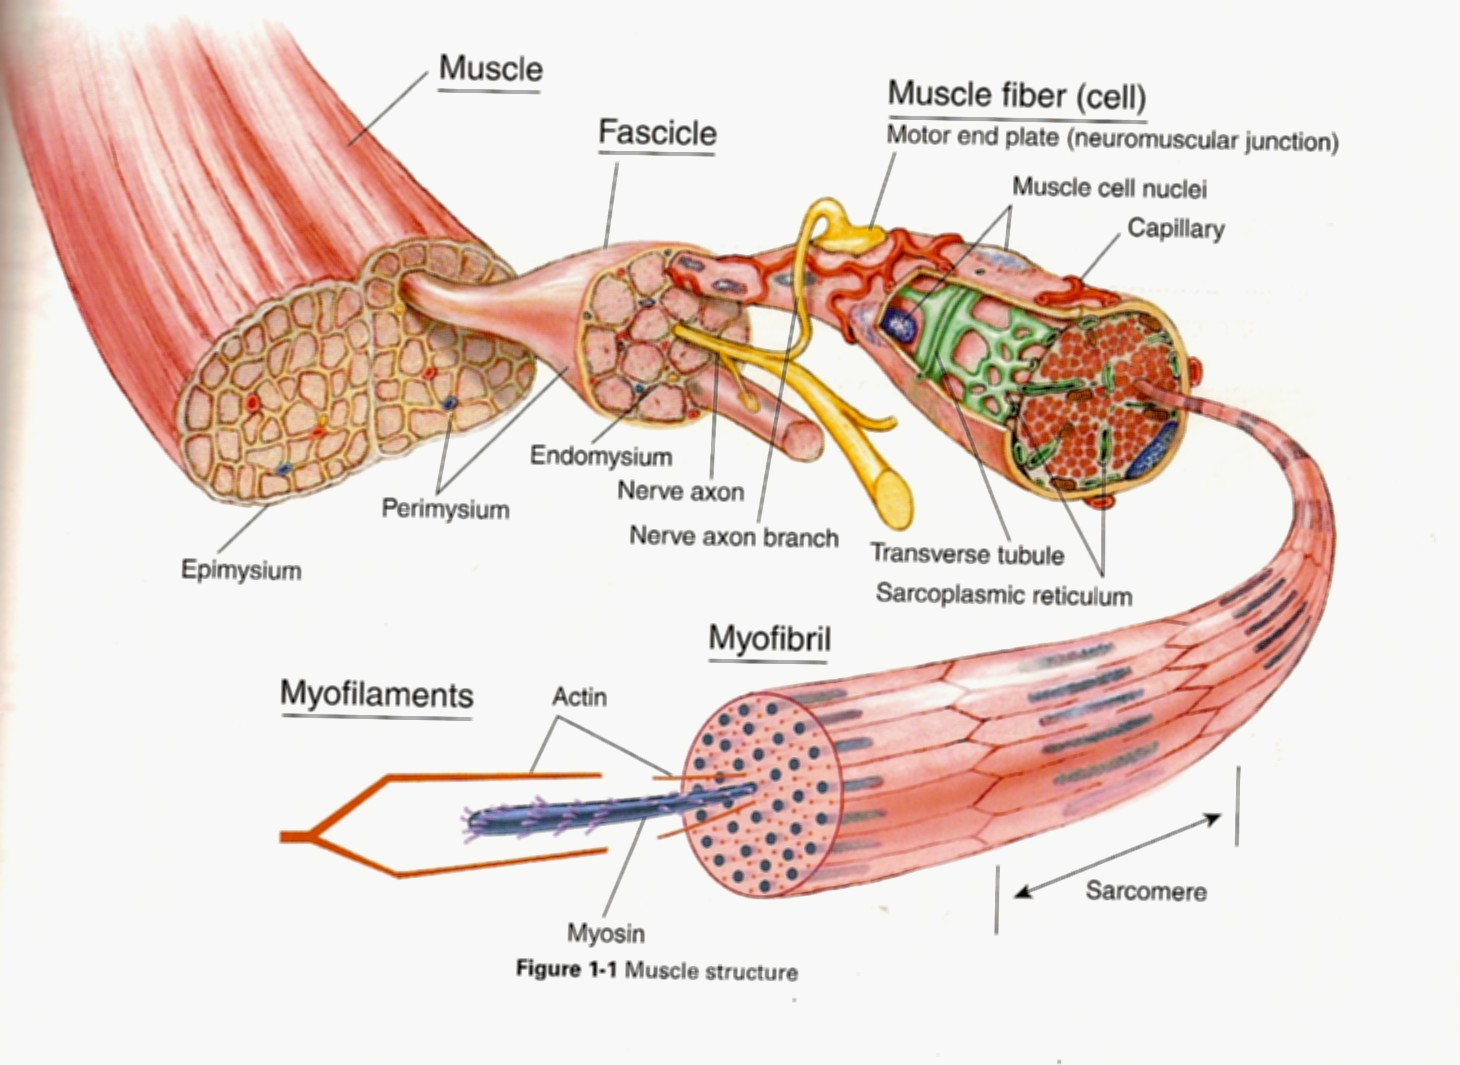
\includegraphics[scale=0.5]{Figures/12_29_0.png} 
 \caption{Illustration de la structure globale du muscle.}
\end{figure}

Dans une myofibre, on trouve de nombreuses myofibrilles liées les unes aux autres, de l'ordre de quelques dizaines, qui occupent la majeure partie de l'espace disponible. Les multiples noyaux sont repoussés en périphérie de la cellule. 

Les myofibres sont regroupées en faisceaux de quelques dizaines de fibres dans un tissu conjonctif composé principalement de différents types de collagène, faisceaux qui sont eux-même regroupés pour former le muscle lui-même. Le tissu conjonctif confère une résistance passive aux muscles et les relie aux tendons qui les fixent sur les os. 

Les capillaires sanguins et les nerfs contrôlant les contractions musculaires sont également encapsulés dans ce tissu conjonctif. 
\subsubsection{Différents types de muscles}

Les fibres musculaires ont toutes une organisation similaire, mais ne sont pas toutes identiques. 
On peut distinguer 2 types majeurs de fibres musculaires : les fibres lentes et les fibres rapides. Les fibres rapides sont mobilisées en premier mais sont plus fatigables que les fibres lentes.  

Les fibres lentes servent aux efforts de longue durée et de faible force, comme par exemple le maintien de la posture, elles se contractent lentement. 
Elles sont riches en mitochondries et en capillaires sanguins, car leur alimentation en énergie se fait principalement par la consommation d'oxygène. 
Les fibres rapides permettent des mouvements puissants, développant une grande force. Elles sont riches en glycogène, dont elles tirent la majeure partie de leur énergie. 





\section{La contraction musculaire}

\subsection{Mécanismes moléculaires}

Le signal de contraction musculaire arrive du système nerveux par un neurone moteur, qui est attaché à une fibre musculaire par la plaque motrice.
Lorsque le signal nerveux est transmis au niveau de la synapse, la membrane de la myofibre est dépolarisée, ce qui aboutit à libérer des ions calcium du Réticulum Sarcoplasmique (l'équivalent pour la cellule musculaire du Réticulum Endoplasmique lisse). 

Les ions calcium libérés se lient à la troponine C, qui est présente sur la tropomyosine qui décore les filaments d'actine dans le sarcomère. La tropomyosine est déplacée sur le filament d'actine, laissant apparaître les sites de liaison à la myosine, qui étaient cachés. 

Les têtes de myosine s'attachent au filament d'actine, puis l'ATP qu'elles contiennent est hydrolysée en ADP+Pi. Le phosphate est ensuite libéré, ce qui provoque un changement de conformation de la tête de myosine, qui avance sur le filament, puis l'ADP est relâchée à son tour, ce qui incline encore plus la tête de myosine. 

À ce moment, les filaments d'actine et les filaments de myosine coulissent les uns par rapport aux autres, ce qui raccourcit la longueur totale du sarcomère. C'est la contraction musculaire. 

En l'absence d'ATP, le phénomène s'arrête à cette étape : les filaments d'actine et de myosine sont attachés les uns aux autres. Le muscle est immobilisé, c'est l'origine de la rigidité cadavérique. 

Lorsqu'elle est présente, l'ATP peut alors remplir le site de liaison laissé vacant par le départ de l'ADP. Cela provoque à nouveau un changement de conformation qui détache la tête de myosine du filament d'actine et la remet dans sa position initiale.

Tant que la concentration en ions calcium est suffisante pour maintenir la tropomyosine dans cette configuration, le cycle attachement-avancée-détachement des têtes de myosine sur l'actine continue, et la fibre musculaire se contracte de plus en plus. 

Lorsque la concentration en calcium diminue car le signal du neurone moteur s'est arrêté, la tropomyosine retrouve sa conformation d'origine, et les myosines ne peuvent plus s'attacher au filament d'actine. 

Pendant la contraction, les protéines du disque M, du disque Z et la titine, qui maintiennent l'alignement des filaments d'actine et de myosine, ont été étirées. Ces protéines peuvent être dépliées pendant la contraction et stocker de l'énergie élastique qui sera rendue lorsque les têtes de myosine seront détachées des filaments d'actine. Lorsque la contraction s'arrête, les filaments coulissent à nouveau dans l'autre sens sous l'action de l'élasticité de ces protéines, et le sarcomère  reprend sa longueur initiale. 


\begin{figure}[p]
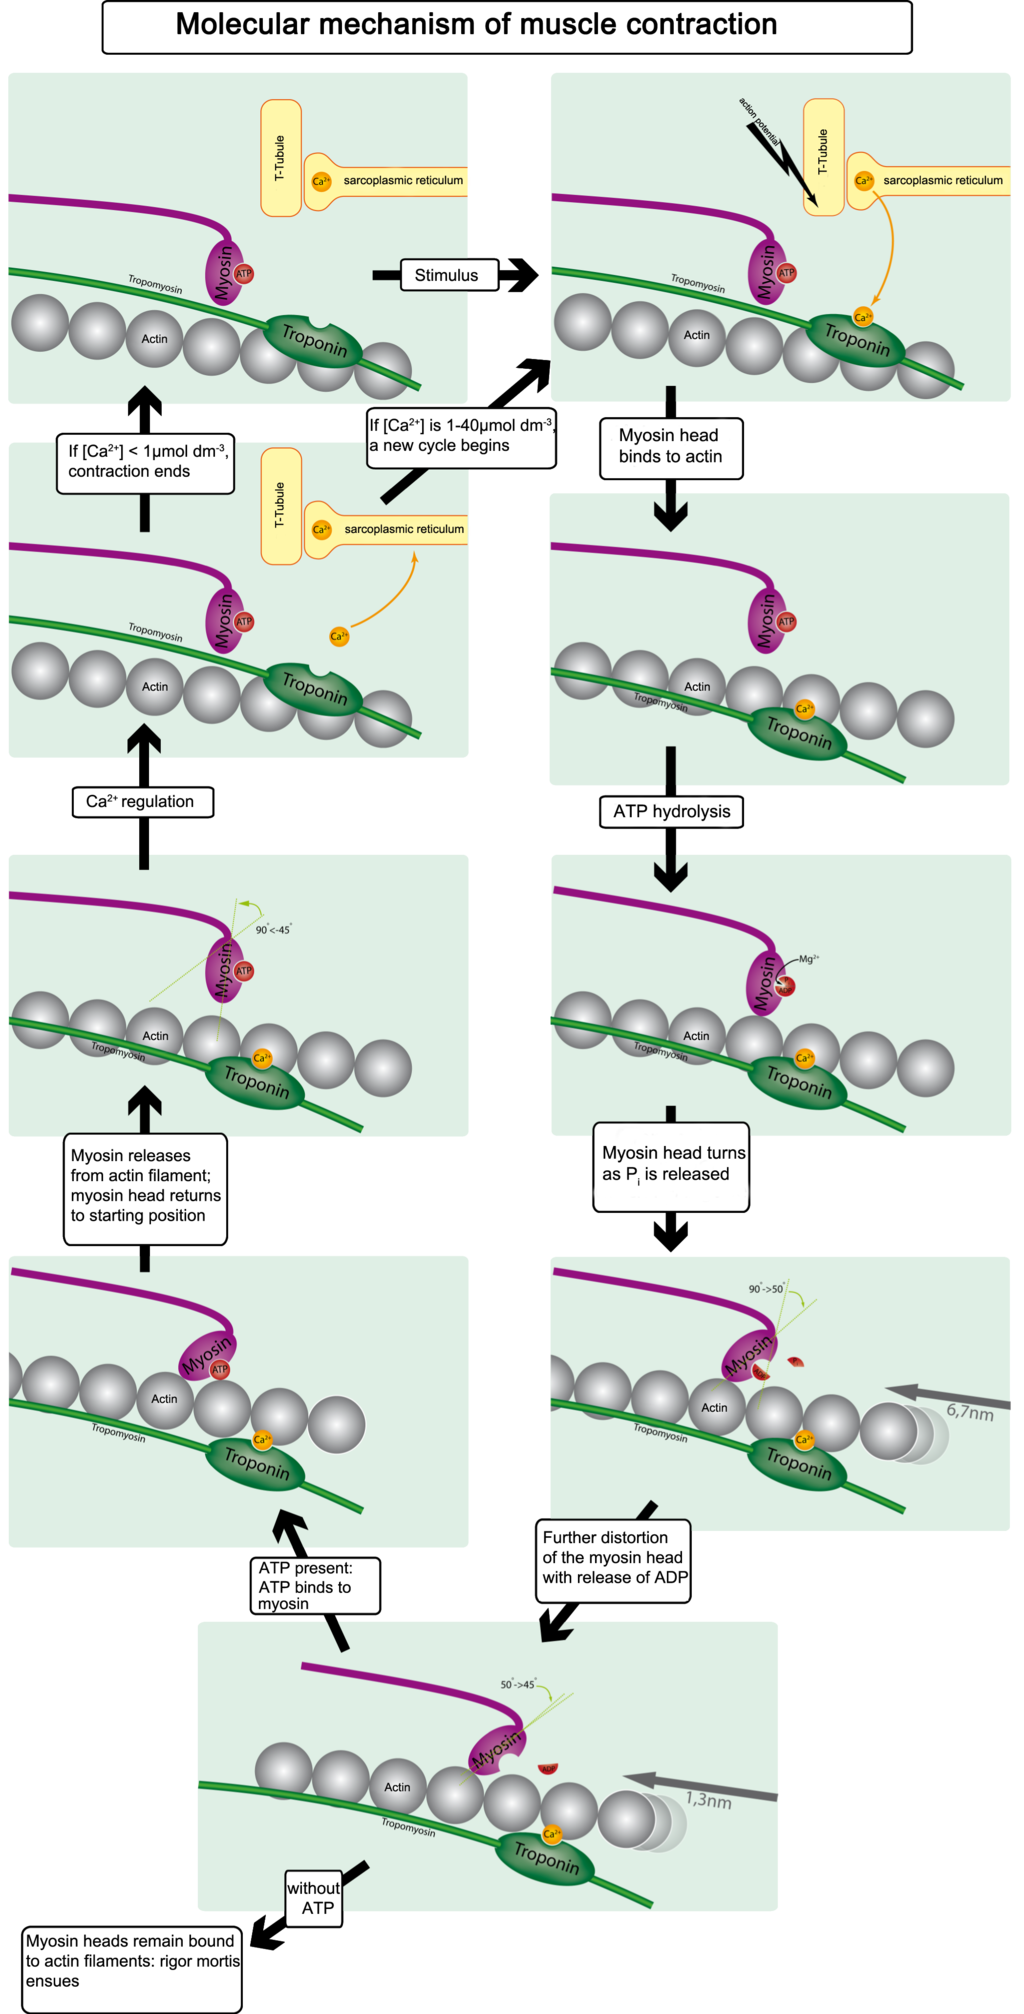
\includegraphics[scale=0.25]{Figures/Contraction.png}
\caption{Illustration du cycle de la contraction musculaire, réalisée par Hank van Helvete (CC BY-SA 2.5)}
\end{figure}
\subsection{Mécanique de la contraction musculaire}
Dans les conditions optimales, une seule cellule musculaire mature humaine peut exercer une force de l'ordre de 0,3 \micro N, et un muscle peut exercer autour de 30N par cm$^2$ de section. 

Le modèle de Hill (\cite{hill_heat_1938}), élaboré bien avant que les mécanismes internes de la contraction musculaire soient connus, permet de relier la vitesse de contraction d'un muscle aux forces qu'il est capable de développer. 

Hill constate que pour un muscle de taille donnée se raccourcissant d'une longueur $x$, l'énergie dissipée dans le muscle est proportionnelle à $x$ : $W_d=ax$. $a$ est proportionnel à la section du muscle (et donc au nombre de myofibres), et comme la force maximale $ P_0$ supportée par le muscle également, le rapport entre les deux  est constant : $$\frac{a}{P_0}=0.25$$

En faisant un bilan d'énergie dans le muscle, on obtient : 
$$ E=W+W_d=Px+ax=(P+0.25P_0)x$$

La puissance totale dissipée vaut alors $(P+a)v$ où $v$ est la vitesse de contraction du muscle, dérivée de $x$ par rapport au temps. 

Hill trouve également que la puissance développée par le muscle est une fonction linéaire du poids qui lui est appliqué, avec $v=0$ quand $P=P_0$. 
La relation devient alors : 
$$ (P+a)v=b(P_0-P)$$
avec $b$ une constante mesurée dans les expériences. 

Cette relation peut se réécrire : 
\begin{equation}
\label{Hill}
(P+a)(v+b)=b(P_0+a)=Cste
\end{equation}
L'équation de Hill relie donc la force que peut appliquer un muscle $P$ à la vitesse de contraction $v$. Plus la contraction est rapide, moins elle peut être forte, au contraire plus elle est lente et plus elle peut développer de force. 

Non seulement la loi de Hill est vérifiée pour les muscles striées, mais elle l'est également au niveau du myoblaste unique (\cite{mitrossilis_single-cell_2009}) et même au niveau d'un unique filament d'actine déplacé par 8 têtes de myosine du muscle squelettique (\cite{debold_slip_2005}), ce qui confirme l'hypothèse de Huxley qui attribue ce comportement aux propriétés du complexe acto-myosine. 

\section{Les cellules satellites, MRTF-A et régulation de la masse musculaire}

Le muscle est un tissu plastique : il peut augmenter ou diminuer sa masse en réponse aux sollicitations mécaniques qui lui sont imposées. Nous en faisons tous quotidiennement l'expérience : la pratique d'activités physiques augmentent la taille de nos muscles, tandis qu'une immobilisation prolongée, comme par exemple suite à une fracture, conduit à une diminution rapide de notre masse musculaire. L'équipe d'Athanassia Sotiropoulos à l'Institut Cochin, avec laquelle nous avons collaboré, a caractérisé le rôle central de SRF dans ce phénomène. 

Entre la lame basale et les myofibres, on peut trouver des cellules satellites, qui contrairement aux autres cellules présentes dans le muscle, sont moins engagées sur la voie de différenciation et peuvent toujours proliférer. Les myoblastes C2C12 et primaires sont issues des cellules satellites prélevées sur des souris. Les cellules satellites sont responsables de la réparation et de la croissance des muscles adultes. 
En effet, les myofibres sont des cellules qui ne se reproduisent plus, et après les deux phases de création de myofibres pendant la vie embryonnaire, le nombre de fibres musculaires reste constant. 
Cependant, lorsqu'elles sont activées en réponse à une blessure ou à une sollicitation importante du muscle, les cellules satellites prolifèrent, et une partie d'entre elles se différencient et fusionnent avec les fibres musculaires. 

Pour étudier la réponse à une stimulation mécanique, des souris ont été soumises à une hypertrophie compensatoire : un des muscles de la patte ne peut plus faire son travail (parce qu’il est dénervé ou que le tendon est sectionné), et les autres sont obligés de compenser son manque d'activité en développant plus de force. En réponse à cette surcharge de travail, SRF est activé dans les myofibres \textit{in vivo} par l'intermédiaire de MRTF-A  (\cite{guerci_srf-dependent_2012}). 
L'activation de SRF dans les myofibres produit un signal paracrine composé d'Interleukines 6, qui encourage la prolifération des cellules satellites, et d'interleukines 4 qui les fait fusionner avec les fibres musculaires. 
Dans les fibres musculaires mutantes où SRF est désactivé, le nombre de noyaux par fibre n'augmente pas, ce qui signifie qu'il n'y a pas de fusion des cellules satellites avec les myofibres. La surexpression d'IL6 chez les mutants restaure la prolifération, mais pas la fusion des cellules satellites. Surexprimer IL4 ou Cox2, qui est en aval de SRF et en amont de l'IL4, permet de restaurer la fusion et l'hypertrophie chez les mutants. 


Au contraire, lors d'une absence de signaux mécaniques induite par la dénervation, l'actine G s'accumule dans le noyau des fibres musculaires et l'activité de SRF diminue (\cite{collard_nuclear_2014}). Le rôle de MICAL-2 est normalement d'exclure l'actine du noyau, et son activité est réduite pendant l'atrophie, ce qui contribue donc à l'accumulation nucléaire d'actine constatée. 
L'accumulation d'actine G dans le noyau favorise l'export de MRTF-A, qui est confiné dans le cytoplasme dans les muscles dénervés. Cela explique le déficit d'activité de SRF, qui ne peut pas être atteint par son cofacteur. 

La désactivation de SRF, l'injection de CCG1423 (drogue inhibant MRTF/SRF), ou l'expression d'une actine non polymérisable conduisent tous à une aggravation de l'atrophie musculaire, ce qui montre que cette voie de signalisation protège l'organisme de la destruction de ses propres muscles. 

Au contraire, l'expression d'une MRTF-A incapable de se lier à l'actine, et donc constitutivement active (sur le modèle de la myocardine), permet de protéger les muscles de l'atrophie induite par la dénervation, ce que ne fait pas la simple sur-expression de MRTF-A GFP. Cependant, si SRF n'est pas fonctionnel, cette protection n'est plus efficace, ce qui prouve que c'est bien le couple MRTF/SRF qui est nécessaire. 


%\end{document}

